\documentclass[12pt,letterpaper]{article}
\usepackage{amsmath}
\usepackage{amsfonts}
\usepackage{amsthm}
\usepackage{mathtools}
\usepackage{cancel}
\usepackage[margin=1in]{geometry}
\usepackage{titling}
\usepackage{graphicx}

\setlength{\droptitle}{-10ex}

\preauthor{\begin{flushright}\large \lineskip 0.5em}
\postauthor{\par\end{flushright}}
\predate{\begin{flushright}\large}
\postdate{\par\end{flushright}}

\title{MAT 167 Project\vspace{-2ex}}
\author{Hardy Jones\\
        999397426\\
        Professor Cheer\vspace{-2ex}}
\date{Winter 2014}

\begin{document}
  \maketitle

  \begin{enumerate}
    \item[Part 1]

      When a problem is overspecified, that is there are more equations than unknowns, we cannot compute an exact solution (or fit the data).
      The Least Squares Approximation attempts to solve this by projecting the problem onto a suitable space and minimizing the error in this projection.

      To put it in symbols, we cannot solve this equation:

      \[\mathbf{A}\vec{x} = \vec{b}\]

      So we approximate it and minimize the error in the process by solving this equation:

      \[\mathbf{A^T}\mathbf{A}\vec{x} = \mathbf{A^T}\vec{b}\]

      In order to fit the to a linear curve we want to solve this equation:

      \begin{align*}
        C + D\vec{x} &= \vec{b} \\
        \begin{bmatrix}
          1 & x_1 \\
          1 & x_2 \\
          \vdots & \vdots \\
          1 & x_m
        \end{bmatrix}
        \begin{bmatrix}
          C \\
          D
        \end{bmatrix}
        &=
        \begin{bmatrix}
          b_1 \\
          b_2 \\
          \vdots \\
          b_m
        \end{bmatrix}
      \end{align*}

      In order to fit the to a parabolic curve we want to solve this equation:

      \begin{align*}
        C + D\vec{x} + E\vec{x^2} &= \vec{b} \\
        \begin{bmatrix}
          1 & x_1 & x_1^2 \\
          1 & x_2 & x_2^2 \\
          \vdots & \vdots & \vdots \\
          1 & x_m & x_m^2
        \end{bmatrix}
        \begin{bmatrix}
          C \\
          D \\
          E
        \end{bmatrix}
        &=
        \begin{bmatrix}
          b_1 \\
          b_2 \\
          \vdots \\
          b_m
        \end{bmatrix}
      \end{align*}

      \pagebreak

      In order to fit the to a cubic curve we want to solve this equation:

      \begin{align*}
        C + D\vec{x} + E\vec{x^2} + F\vec{x^3} &= \vec{b} \\
        \begin{bmatrix}
          1 & x_1 & x_1^2 & x_1^3 \\
          1 & x_2 & x_2^2 & x_2^3 \\
          \vdots & \vdots & \vdots & \vdots \\
          1 & x_m & x_m^2 & x_m^3
        \end{bmatrix}
        \begin{bmatrix}
          C \\
          D \\
          E \\
          F
        \end{bmatrix}
        &=
        \begin{bmatrix}
          b_1 \\
          b_2 \\
          \vdots \\
          b_m
        \end{bmatrix}
      \end{align*}
  \end{enumerate}

  When we use a linear fit, Figure \ref{fig:linear_least_squares}, we get a \textit{very} rough fit of the data. It seems to just barely provide enough information to find a given datum, and when it does, the error is still fairly large.

  \begin{figure}[h]
    \centering
    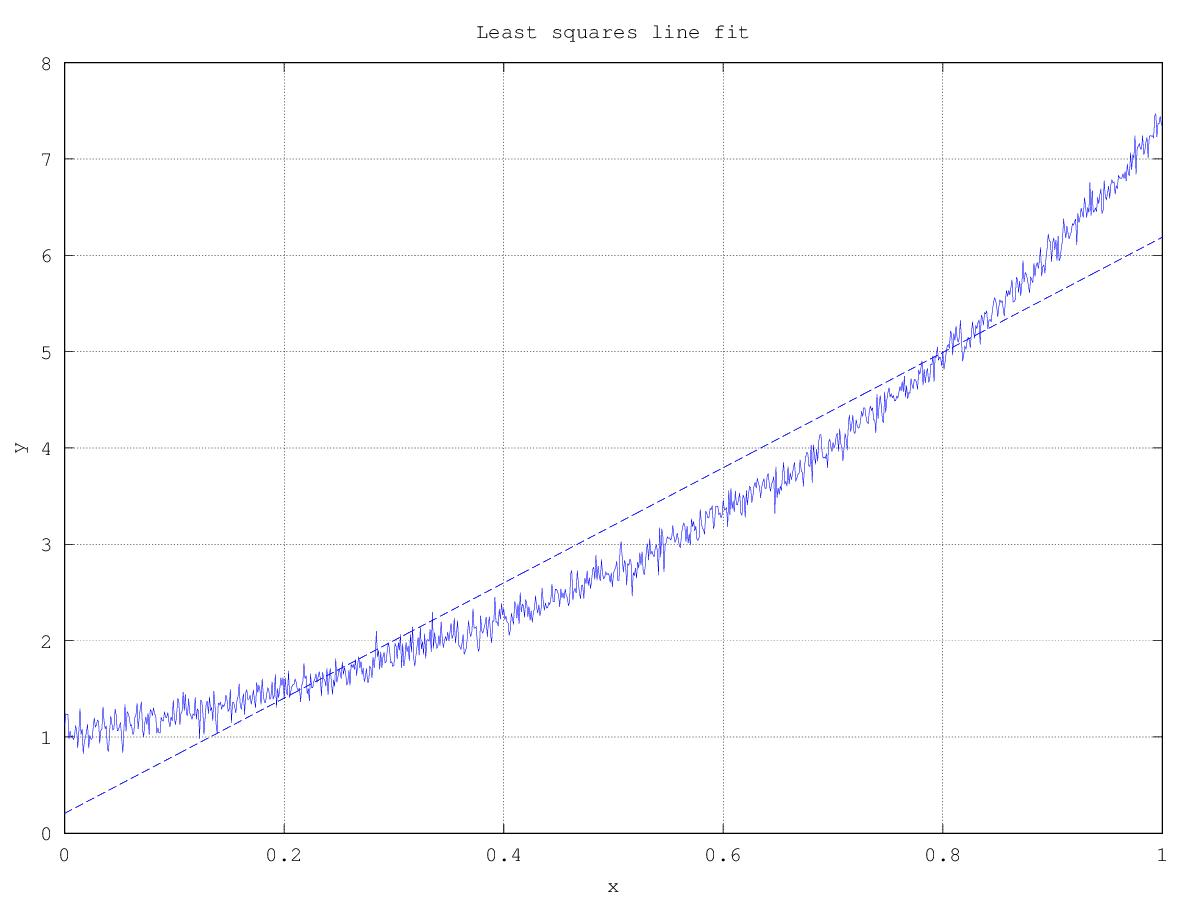
\includegraphics[width=0.95\textwidth]{least_squares_linear.jpg}
    \caption{Linear Least Squares}
    \label{fig:linear_least_squares}
  \end{figure}

  \pagebreak

  When we use a parabolic fit, Figure \ref{fig:parabolic_least_squares}, we see that our solution much better describes the problem.
  With the linear fit, it appears as if we're saying the, ``The data goes this way''.
  With the parabolic fit, it appears more as though we're saying, ``the data is in this region, give or take''. There are still some points where the curve is above and below the ``meat'' of the data. This is a much better approximation because our error has decreased dramatically, but we can still do better.

  \begin{figure}[h]
    \centering
    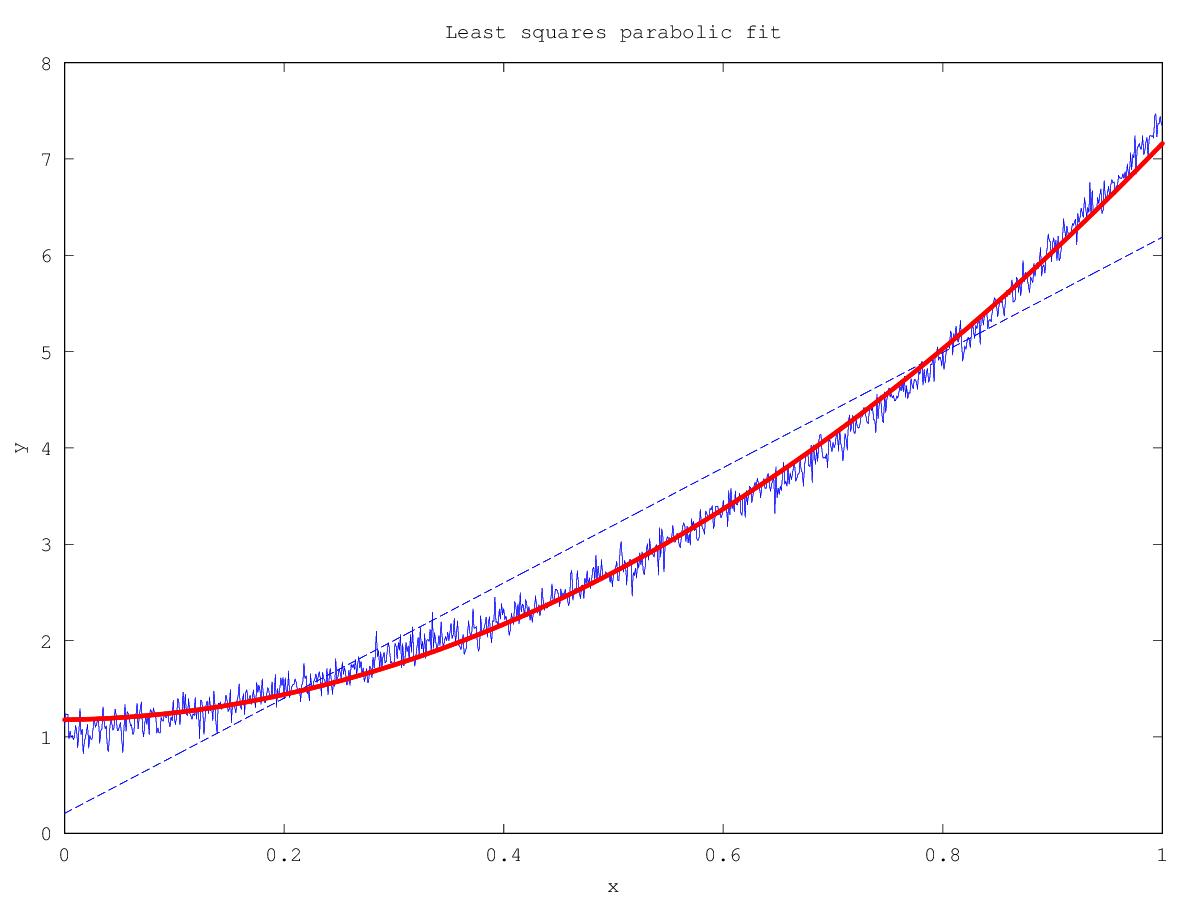
\includegraphics[width=0.95\textwidth]{least_squares_parabolic.jpg}
    \caption{Parabolic Least Squares}
    \label{fig:parabolic_least_squares}
  \end{figure}

  \pagebreak

  When we use a cubic fit, Figure \ref{fig:cubic_least_squares}, we see a curve that very nearly describes the attitude of the data. It never seems to deviate too far from the ``slope'' of the data. The error has been reduced even further in comparison with the parabolic fit.

  \begin{figure}[h]
    \centering
    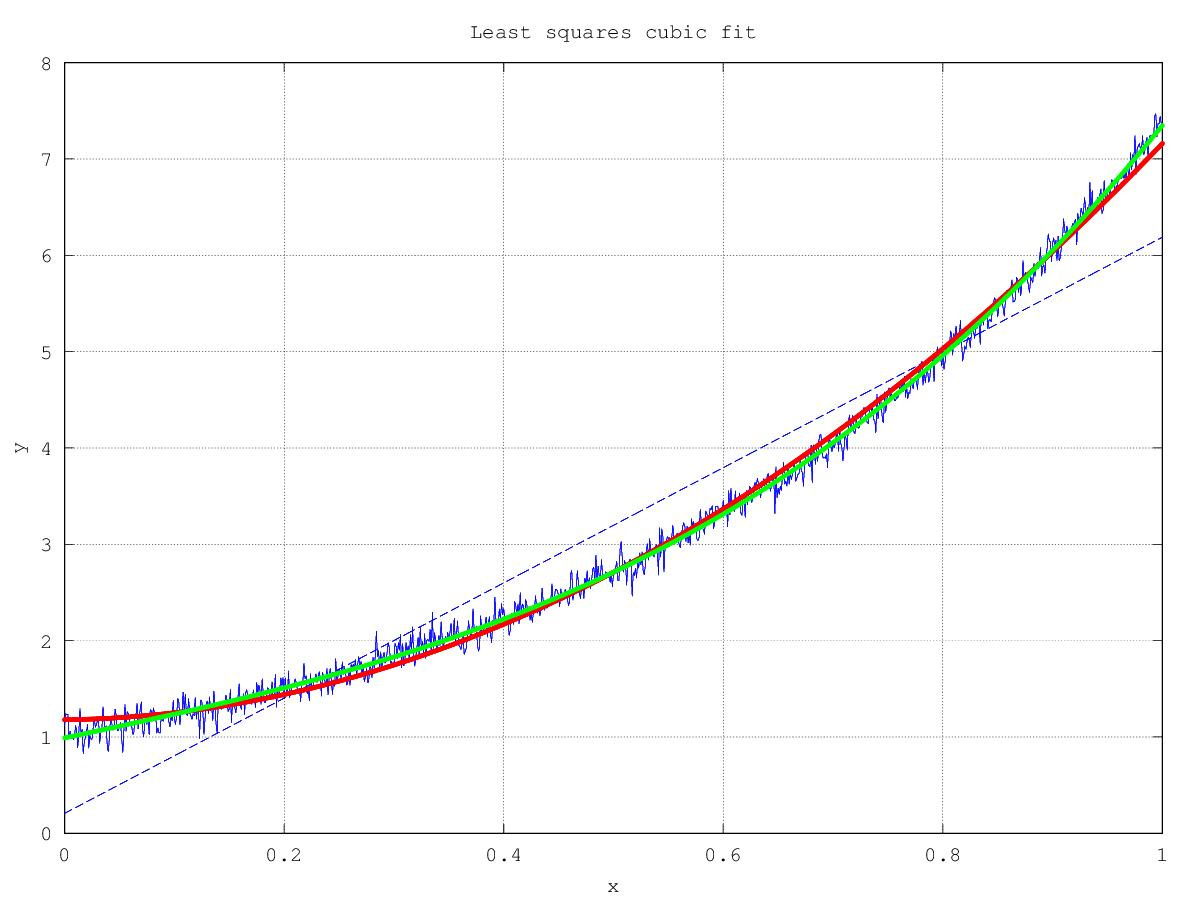
\includegraphics[width=0.95\textwidth]{least_squares_cubic.jpg}
    \caption{Cubic Least Squares}
    \label{fig:cubic_least_squares}
  \end{figure}

  In each of these examples, the error is the vertical distance between a datum point and the curve.

  \begin{figure}[h]
    \centering
    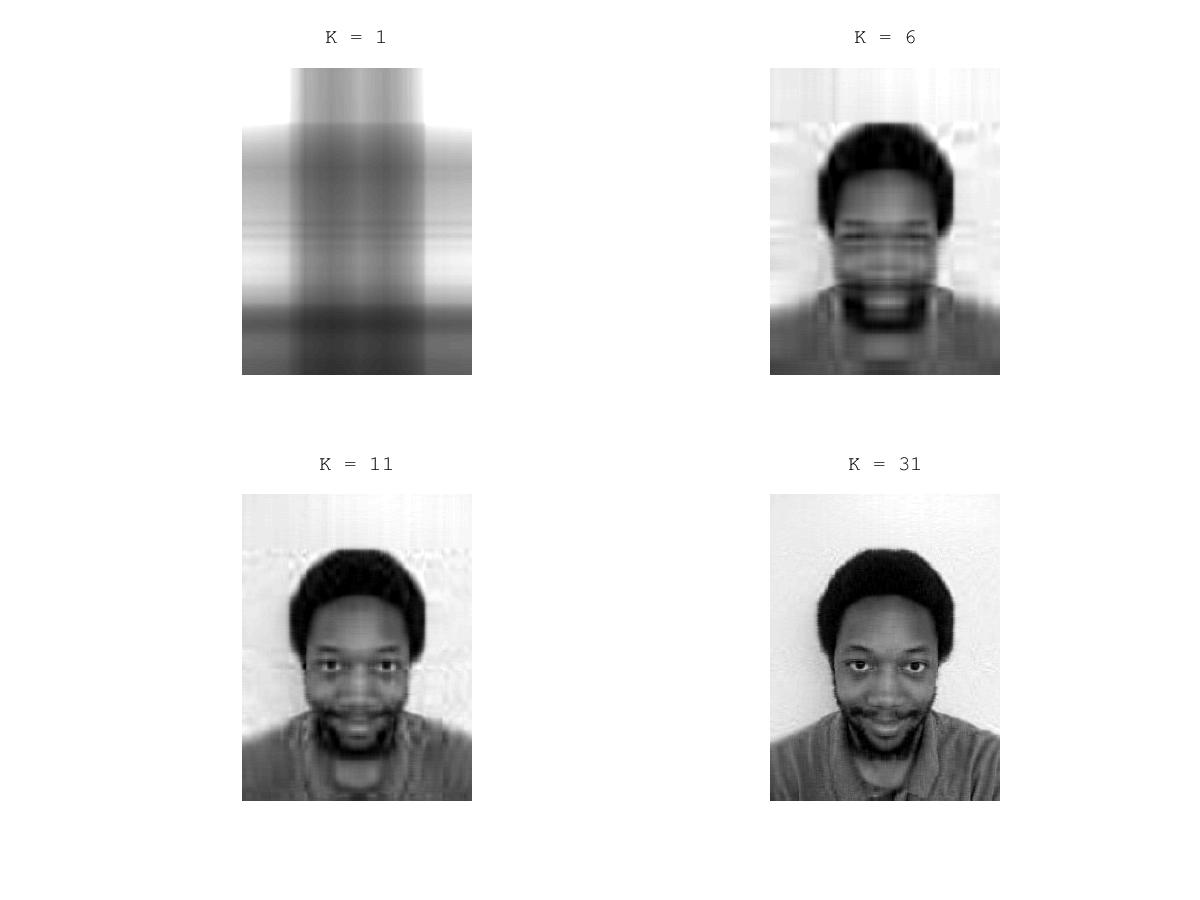
\includegraphics[width=0.95\textwidth]{rank_k.jpg}
    \caption{Rank K Approx.}
    \label{fig:rank_k}
  \end{figure}

\end{document}
